\documentclass[twoside,twocolumn,a4paper]{article}

\usepackage{blindtext} % Package to generate dummy text throughout this template 

\usepackage[sc]{mathpazo} % Use the Palatino font
\usepackage[T1]{fontenc} % Use 8-bit encoding that has 256 glyphs
\linespread{1.15} % Line spacing - Palatino needs more space between lines
\usepackage{microtype} % Slightly tweak font spacing for aesthetics

\usepackage[english]{babel} % Language hyphenation and typographical rules

\usepackage[hmarginratio=1:1,top=32mm,columnsep=20pt]{geometry} % Document margins
\usepackage[hang, small,labelfont=bf,up,textfont=it,up]{caption} % Custom captions under/above floats in tables or figures
\usepackage{booktabs} % Horizontal rules in tables

\usepackage{subcaption}
\usepackage{graphicx}

\usepackage{lettrine} % The lettrine is the first enlarged letter at the beginning of the text
\usepackage{color}
\usepackage{enumitem} % Customized lists
\setlist[itemize]{noitemsep} % Make itemize lists more compact

\usepackage{abstract} % Allows abstract customization
\renewcommand{\abstractnamefont}{\normalfont\bfseries} % Set the "Abstract" text to bold
\renewcommand{\abstracttextfont}{\normalfont\small\itshape} % Set the abstract itself to small italic text

\usepackage{titlesec} % Allows customization of titles
\renewcommand\thesection{\arabic{section}} % Roman numerals for the sections
\titleformat{\section}[block]{\large\scshape}{\thesection.}{1em}{} % Change the look of the section titles
\titleformat{\subsection}[block]{\large}{\thesubsection.}{1em}{} % Change the look of the section titles

\usepackage{fancyhdr} % Headers and footers
\pagestyle{fancy} % All pages have headers and footers
\fancyhead{} % Blank out the default header
\fancyfoot{} % Blank out the default footer
\fancyhead[C]{Wind Farm Power Regulation $\bullet$ May 2016} % Custom header text
\fancyfoot[RO,LE]{\thepage} % Custom footer text

\usepackage{titling} % Customizing the title section

\usepackage{hyperref} % For hyperlinks in the PDF

\usepackage{amsmath}

\usepackage{placeins}

\setlength{\droptitle}{-4\baselineskip} % Move the title up

\pretitle{\begin{center}\Huge\bfseries} % Article title formatting
	\posttitle{\end{center}} % Article title closing formatting
\title{Wind Farm Power Regulation Using Yaw Control and Axial Induction Control} % Article title
\author{%
	\textsc{Niels van Duijn, Jurriaan Govers, Luuk van Hagen}\\
	\textsc{Jochem Hoorneman, Max van Leeuwen}\\%\thanks{A thank you or further information} [1ex] % Your name
	\normalsize TU Delft \\ % Your institution
	%\normalsize \href{mailto:j.a.govers@gmail.com}{j.a.govers@gmail.com} % Your email address
	%\and % Uncomment if 2 authors are required, duplicate these 4 lines if more
	%\textsc{Jane Smith}\thanks{Corresponding author} \\[1ex] % Second author's name
	%\normalsize University of Utah \\ % Second author's institution
	%\normalsize \href{mailto:jane@smith.com}{jane@smith.com} % Second author's email address
}
\date{\today} % Leave empty to omit a date
\renewcommand{\maketitlehookd}{
\begin{abstract}
	\noindent With wind energy gaining importane on the energy marked, wordt optimaal gebruikmaken van de beschikbare resorces, zowel als betrouwbaarheid en stabielitijd van steeds groter belang. Nowadays, more and more of the wind energy is generated in windfarms. These farms have the advantages of beeing cheaper in instalation aswell as maintanance. However, the currend controll method(gready controll) is far from optimal, and only takes power into account. This paper combines the use of 2 other types of controll methods (yaw and axial induction controll) to find the optimal running procedure of a windfarm. Decresing the damaging loads on the turbines, while beter regulating the poweroutput. At the same time making wind energy cheaper aswell as increasing its stabillitie. Making windenergy ready for the future.
	
\end{abstract}
}

\begin{document}

\maketitle

\section{Introduction}
\lettrine[nindent=0em,lines=3]
With an increasing role of wind energy production new challenges arise\cite{Nat2016}. In the EU, wind power capacity has increased sixfold, from 2,4\% market share in 2000 to 15,6\% in 2015, overtaking hydro as the third largest power generation capacity \cite{EWEA2016}. To efficiently use resource rich locations and minimize the cost of energy, wind turbines are constructed in close proximity of each other, creating wind farms. In operation, an area of decreased wind velocity and increased turbulence occurs behind the turbine, called a wake. Overlap of the wake with a downstream turbine causes loss of power and increased fatique loads \cite{Boersma2017, Wilson2017, Dijk2016, Fleming2014, Zalkind2016}. 

While the market becomes more dependent on wind energy, it is important for wind farms to be able to meet the demands of the power by regulating its output \cite{Tande2003}. Wind farm power regulation is needed to prevent, for example, an overloaded energy grid \cite{Hansen2014}.  \\
\indent Currently, most wind farms operate based on 'greedy control', i.e. each individual turbine is set to run for maximum power production, neglecting wake interaction. Previous studies on this effect mainly focused on maximizing the power output of the wind farm while minimizing loads \cite{Wilson2017, Dijk2016, vanDijk2016}. In this paper the focus is shifted to power regulation and loads minimization. Therefore two methods will be discussed, yaw control and axial induction control. The loading is a function that depends on four variables, $D_{wake}$, $U_{fs}$, $\gamma$, and $y _{C2C}$. \\
\indent Yaw control can be used as a method to redirect a wake from a downstream turbine. This reduces the loads and increases the power output of the downstream turbine. A disadvantage of yawing is a possible increase of loads on the yawed turbine, and thus reducing its lifespan \cite{Zalkind2016,Kanev2017}. Furthermore, under unfavorable conditions it can result in an asymmetrical overlap of the wake on the downstream turbine, significantly increasing the loads on this turbine \cite{Wilson2017,Dijk2016}. \\
\indent Axial induction control influences the power output of a turbine by means of the blade pitch angle and generator torque. The axial induction factor reflects the relation between the free stream wind velocity and the wind velocity leaving the rotor. By varying the axial induction factor of a wind turbine, the power output can be controlled. Moreover, the axial induction factor is proportionally linked to the size of the wake and thus influences overlap between a wake and a downstream turbine.  

This paper is divided into four sections, section 1 being the introduction. Section 2 describes the data generation and optimization methods. In section 3 the results of the optimization will be presented. Finally, section 4 draws a conclusion and discusses the results. Furthermore, recommendations for future studies are given.


\section{Method} \label{sec:method}
	The optimization of power regulation while minimizing loads, requires a model that can describe the power output and the loads of a wind farm. The implementation of this is described in this section. \newline
	An overview of the optimization procedure used can be seen in Figure \ref{fig:optim}.
	The power output of a wind farm as well as the wake propagation in this wind farm are calculated using the FLORIS model (Section \ref{sec:floris}). Given a certain inflow profile the program FAST calculates the out of plane bending moments on a turbine. With the program MLife these bending moments are converted to a Damage Equivalent Load (DEL), which is a measure for the lifespan of a wind turbine \cite{MLife}. Both FAST and MLife are covered in Section \ref{sec:fast}. These DELs are pre-calculated for different situations which are determined by four parameters and then stored in a look-up-table (LUT). \newline


	To realize power regulation and minimizing loads by yaw control and axial induction, it is necessary to know the effects of different flow conditions on the total power of the wind farm and the effect of different flow conditions on the loads for each of the turbine. Moreover, there need to be an optimizer which executes the optimization to approach a set value for the power and to minimize the loads.\newline


	The total power of the wind farm is calculated with the FLORIS-model. Besides, FLORIS is able to adjust the turbine configurations, the axial induction and yaw position.  
	The effect of the wind flow on a turbine, regarding the loads, are given by the programs FAST and MLife. The output of these programs are Damage Equivalent Load values (DELs), which are a measure of equivalent load damage to the turbine concerning the material properties.\cite{Chougule2016} These DELs are calculated for a different set of wind and turbine conditions and are stored in a look-up table(LUT).

	
	The optimizer takes the desired power production of the wind farm as an input. It used the configurations of the turbines from FLORIS to find the corresponding DEL values in the look-up table. If the configurations of the turbines are an improvement compared to the previous one, i.e. a improved power control or a reduce in the loads, FLORIS will save this turbine configurations. An overview of the optimization procedure is shown in Figure \ref{fig:optim}. 
	\\
	\\
	In the following sections, different models and model steps, used to perform the optimization, are explained:
	
	
	
	\begin{figure}
		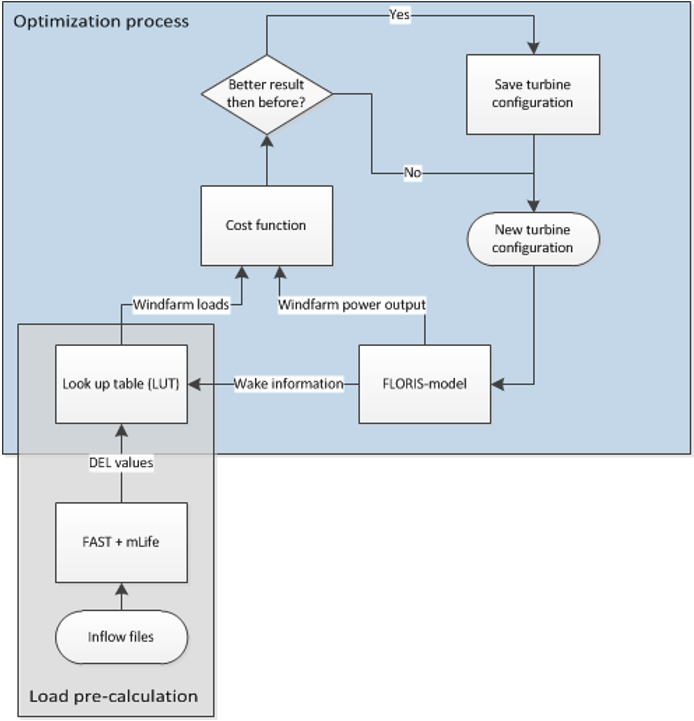
\includegraphics[width=\linewidth]{./Figures/OptimizationProcess.png}
		\caption{Overview of the optimization procedure.}
		\label{fig:optim}
	\end{figure}


  


%\noindent

\subsection{FLORIS} The FLORIS, or FLOw Redirection and Induction in Steady state, model is used for the generation of wake propagation and power output data of windfarms as a function of the yaw misalignment and the axial induction\cite{Gebraad2016}.
FLORIS is a relative accurate model\cite{Dijk2016} with a relatively low computation time, since it is a parametric model fitted to high-fidelity data from a computational fluid dynamics simulation. 

\subsubsection{Wake modelling}
\label{wakemodel}
%As can be seen in Figure \ref{fig:wake}, 
FLORIS generates a wake model which divides the wake into three different zones as shown in Figure\ref{fig:wake}. These zones are as the near wake, the far wake, and the mixing zone, and are denoted by $q$. Each zone has its own diameter and wind speed, which are calculated by FLORIS using Equations(\ref{eq:Dw} to \ref{eq:c}). 


\begin{figure}
  	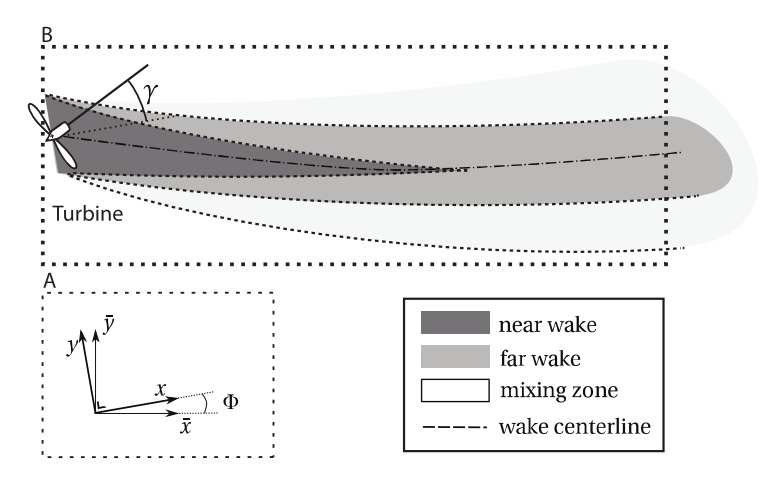
\includegraphics[width=\linewidth]{./Figures/WakeFLORIS.png}
  	\caption{Simplified top view representation of a wake of a turbine by FLORIS.\cite{Gebraad2016}   }
	\label{fig:wake}
\end{figure}

The size of the wake diameter is calculated using Eq \ref{eq:Dw}. let the $D_i$ denote the rotor diameter of the $i${\textsuperscript{th}} turbine, $k_e$ a coefficient that describes expansion of the zones, and $m_{e,q}$, the expansion factor as used by Gebraad\cite{Gebraad2016}. The size of the wake diameter $D_{w,q,i}$ increases proportionally to the downwind distance ($x$). 
\begin{equation}
\label{eq:Dw}
D_{w,i,q}(x) = max({D_i + 2k_em_{e,q}([x - X_i],0} )
\end{equation}
The wake velocity depends on the downwind distance $(x)$ as well. As shown in Eq \ref{eq:Uw}, is the wake velocity an argument of the wake decay coefficient $c(x,y)$ (<--). This wake decay coefficient is multiplied by the axial induction factor and subtracted from the free stream velocity $U_i$. The axial induction factor is a value for the decrease in wind velocity behind a turbine relative to its own rotor speed. The wake decay coefficient describes the decay of velocity for each wake zone and is defined in \ref{eq:c}. The model parameter $M_{U,q}$, which depends on the wake zone and the yaw angle, is calculated by Gebraad.\cite{Gebraad2016}   

\begin{equation}
\label{eq:Uw}
U_{w,i}(x,y) = U_i\left( {1-2a_ic_i(x,y)} \right)
\end{equation} 

\begin{equation}
\label{eq:c}
c_{i,q}(x) = \left[ \frac{D_i}{D_i + 2k_em_{U,q}(\gamma_i)[x - X_i]} \right]^2
\end{equation}




%\noindent

\subsection{FAST \& MLife} FAST is a programming tool for the simulation of dynamic (load) responses of wind turbines (by NREL) \cite{Jonkman2005}. By evaluating a flow field, FAST computes the bending moment of a blade. Since the bending moment of a blade does not give direct information about the effect on the life-cycle time of a turbine, the program MLife is used to convert the bending moment to damage equivalent loads (DELs). (these DELs are better why??)


\begin{figure}
  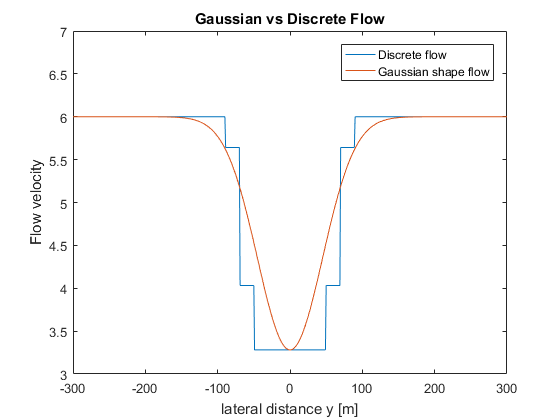
\includegraphics[width=\linewidth]{./Figures/PlotGausDiscWakeDWake180U6yaw0.png} %Plot with Gauss vs Discr flow, Dwake = 180, u_mean = 6, yaw = 0
  \caption{Discrete wake versus Gaussian wake} %for Dwake = 180 m, U = 6 m/s, and yaw = 0
  \label{fig:disgaus}
\end{figure}

%\noindent

\subsubsection{Inflow files, Flow field}
FAST uses wind turbine specifications as well as wind flow situations to generate load data. These flow files are 
\paragraph{Gaussian wake}
FLORIS describes a discrete flow field of a wake, with three zones. The flow field of the wake in FLORIS is calculated with equations (\ref{eq:Dw} to \ref{eq:c}). The wake is divided into three zones as described in paragraph \ref{wakemodel}. A real wake, however, does not have these discrete zones. To create a more fluent transition between the different wake-zones a Gaussian distribution of the flow field is chosen \cite{Bastankhah2016}. The difference of wake shape between a Gaussian and discrete shape can be seen in Figure \ref{fig:disgaus}.  The Gaussian distribution is calculated as follows: 

\begin{equation}
\label{eq:gaus}
G(y, z) = A [e^{-(\frac{y^2}{2\sigma_y} + \frac{z^2}{2\sigma_z})}]
\end{equation}
The amplitude of the Gaussian, $A$, is set to be equal to the velocity loss of the inner wake zone, $U_{w,1}$, as FLORIS models it(!!verwoording mag anders). $\sigma_y$ and $\sigma_z$ reflect the Gaussian standard deviation in horizontal and vertical direction, respectively. These standard deviations are related to the outer wake zone $D_{w,i,q=3}$ following Equation \ref{eq:sigm},
\begin{equation}
\label{eq:sigm}
\sigma_y,\sigma_z = D_{w,i,q=3}/n 
\end{equation}
\\
Where fit parameter $n$ can be modified to change the width of the Gaussian. Consequently, making it possible to fit the Gaussian to the wake zones of FLORIS. (Figure \ref{fig:disgaus})
(clearly note the relation between the gausian and the wakes from FLORIS)

\paragraph{Wind shear} \label{sec:windshear}
Wind shear can cause an important difference in velocity speeds between the rotor hub height, the end of the rotor blades at their highest points and the end of the rotor blades at their lowest point \cite{Firtin2011}.  The velocity distribution is calculated with, 
\begin{equation}
\label{eq:shear}
v = v_{ref} \left[\frac{h}{h_{ref}}\right]^\alpha
\end{equation}
where $v$ and $v_{ref}$ are the velocity at heights $h$, and $h_{ref}$  respectively. Value $\alpha$ is the wind shear coefficient which depends on different factors. Coefficient $\alpha$ is fixed at value 0.1, reflecting a terrain type close to ocean and smooth ground \cite{Firtin2011}. The wind shear is implemented in the flow field. The difference between a flow field with and without wind shear can be seen in Figure \ref{fig:windshear}

\begin{figure}
	\centering
	\begin{subfigure}[b]{0.50\textwidth}
		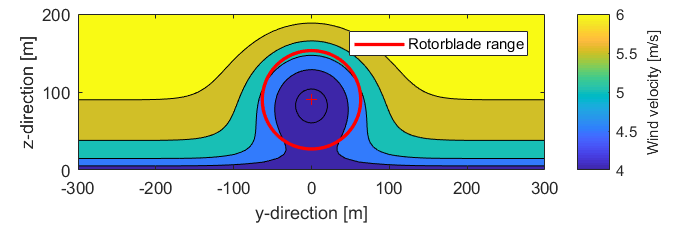
\includegraphics[width=\linewidth]{./Figures/PlotwithshearU6D220.png} %Plot with windshear u_mean = 6
		\caption{Flow field with wind shear.}
		\label{fig:windsh}
	\end{subfigure}
	
	\begin{subfigure}[b]{0.50\textwidth}
		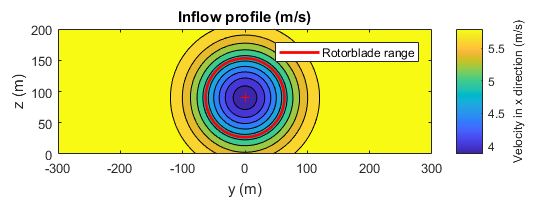
\includegraphics[width=\linewidth]{./Figures/PlotwithoutshearU6D220.png} %Plot without windshear u_mean = 6
		\caption{Flow field without wind shear}
		\label{fig:nowindsh}
	\end{subfigure}
	
	\caption[Two Gaussian flow fields]{Gaussian wind fields with a free stream velocity of 6 $m/s$ at a height of 90 $m$. The outer diameter of de wake is 220 $m$ and the diameter of the rotor blades is 126.4 $m$.}
	\label{fig:windshear}
\end{figure}




\begin{table}[h]
	%\renewcommand{\arraystretch}{1.3} 
	\caption{Overview of the minimum value, maximum value, and step size of the parameters, diameter of outer wake zone (Dwake), free stream wind speed (U), yaw of the turbine (yaw), and the center to center distance between the center of the turbine and the center of the wake (y wake).}
	\centering
	\label{tab:pars}
	\begin{tabular}{lccc}
		\hline
	 	& Minimum & Maximum & Step-size \\ 
		\hline
		Dwake & 180 & 330 & 25 \\
		U & 6 & 8 & 2 \\
		yaw & -30 & 30 & $^*$ \\
		y wake & -250 & 250 & 10 \\
		\hline
	\end{tabular}
$^*$Input values for yaw are [-30, -10, -5, 0, 5, 10, 30].
\end{table}

%\noindent
\subsection{LUT} \label{sec:lut}
 To reduce computational time during optimization a look-up table (LUT) is created. The LUT is created using FAST and MLife, and it contains a a large number of DEL values for a wide variety of wind field conditions on a wind turbine.
These different conditions are described by the ranges of the parameters, which can be seen in Table \ref{tab:pars}. The parameters are wake characteristics which can be extracted from FLORIS. The parameters chosen for the LUT are:\begin{itemize}
	\item the free stream wind speed, U
	\item the outer diameter of the wake, Dwake
	\item the yaw of the turbine, yaw  
	\item the center to center distance between the turbine and the wake, y wake 
\end{itemize}   
 To save calculation time, the LUT parameters are discretized, given each parameter a certain step-size. This step-size is chosen such that interpolation will give a representative result. For each parameters step-sizes are selected, as shown in Table \ref{tab:pars}. With the use of the pre-calculated LUT, online optimization can be realized.



 This paper uses the wake diameter as a parameter to characterise the wakes. However, as stated before are the diameter of the wake, the downwind distance and the windspeed reduction behind the turbine(Udef) related by fitting equations. This means that the distance and the Udef could have been used as parameter just as well. The choice for the diameter comes since Floris searches for the best fit of the shape of a wake in the LUT data. And the diameter gives a more direct interpretation of the shape of the wake than the others do, subsequently meaning that the diameter comes more intuitively.

 
 

%\noindent
\subsection{Optimization} \label{sec:optimization}
To optimize for power reference tracking and load minimization, a game-theoretic approach was used.\cite{Marden2013} The optimization algorithm searches for the optimal yaw and axial induction settings of each individual turbine. These can influence the power and loads significantly, so both are combined in a cost function. \cite{Marden2013}\cite{Dijk2016} 

\subsubsection{Cost Function} \label{sec:costfunction}
The cost function depends on two variables: a normalized power and a normalized load variable. To achieve the optimal yaw and axial induction settings a mixed-objective cost function is defined as follows:

\begin{equation}
\begin{aligned}
J(P,DEL) = c*((P_{ref}-P(a_i,\gamma_i))/P_{bw})^2  + \\
(1-c)*DEL(a_i,\gamma_i)/DEL_{base}
\end{aligned}
 \label{eq:costf}
\end{equation}
Where $c$ is the tuning parameter for the optimization between power and loads and $P_{ref}$ is the desired power output of the wind farm. $P_{bw}$ and $DEL_{base}$ are the power and loads baselines respectively, to create normalized variables.
\newline
To execute the optimization, the cost function has to be minimized. To obtain power production close to the reference, the power part of the cost function is a quadratic difference. As a result values much larger than the reference are heavily penalized, whereas the power crosses $P_{bw}$ the emphasis shifts to the loads.

\subsubsection{Game Theory} \label{sec:gametheory}
The game-theoretic approach uses random perturbations for the yaw angles and the axial induction to optimize the cost function. When new values for yaw and axial induction settings give an improvement regarding the cost function, the settings are saved and the process will be repeated with the new settings. Because of the fact it uses random perturbations, the game theoretic approach is an adequate optimizer to find the global minimum of the cost function.\cite{Dijk2016}




	
\section{Results}

In this chapter different results are shown.

\subsection{Look-up-table}
As an example of the DEL values stored in the LUT a visualization of a slice with a $D_{wake}$ of 230m and a $U_{fs}$ of 8m/s is shown in figure \ref{fig:LUTslice}. Slices for different $D_{wake}$ and $U_{fs}$ look similarly.

\begin{figure}
	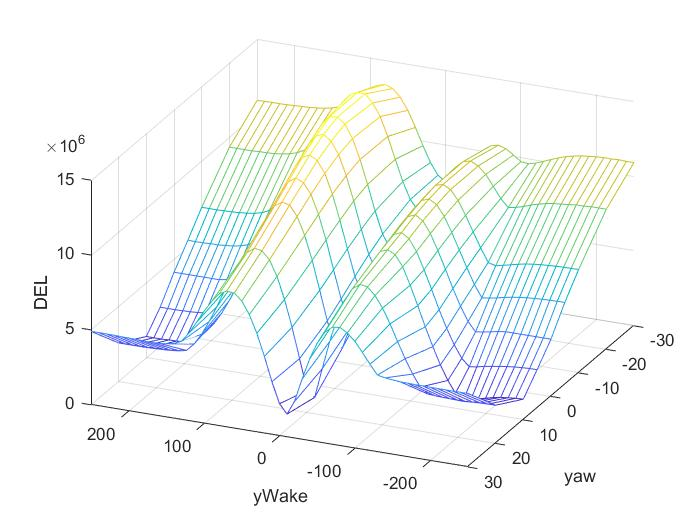
\includegraphics[width=\linewidth]{./Figures/LUTslice_Dw230_Ufs8.jpg}
	\caption{Slice of the LUT with a $D_{wake}$ of 230m and a $U_{fs}$ of 8m/s }
	\label{fig:LUTslice}
\end{figure}

\subsection{Optimization}
The optimization script is run on a set of nine wind turbines which are place in a 3-by-3 grid. As a reference 'greedy control' is used. To determine the maximum power the nine wind turbines can deliver an optimization is executed taking only power into account. See table \ref{tab:reference} for the power and DEL values for both these situations. \newline
To show the optimization script in action five cases are evaluated. Each case has its reference power $P_{ref}$ set as a percentage of the maximum power. In figure \ref{fig:optimization90pct} power and DEL values during optimization with a reference power of 90\% are shown. Figure \ref{fig:config90pct} shows the final turbine configuration for this optimization run. \newline
Figure \ref{fig:optimizationTrends} shows the DEL values for different reference powers.


\begin{table}[h]
	\caption{Power and DEL values for greedy control and power-only optimization}
	\centering
	\label{tab:reference}
	\begin{tabular}{lccc}
		\hline
		& Greedy control & Power-only \\ 
		\hline
		Power [MW] & 12.42 & 13.22 \\
		DEL value [-] & 5.94E7 & - \\
		\hline
	\end{tabular}
\end{table}

\begin{figure}
	\includegraphics[width=\linewidth]{./Figures/{Configuration_Pref11.9}.jpg}
	\caption{Turbine configuration after optimization with $P_{ref}$ at 90\% }
	\label{fig:config90pct}
\end{figure}

\begin{figure}
	\includegraphics[width=\linewidth]{./Figures/{Optimization_Pref11.9}.jpg}
	\caption{Loads and power during optimization with $P_{ref}$ at 90\% }
	\label{fig:optimization90pct}
\end{figure}

\begin{figure}
	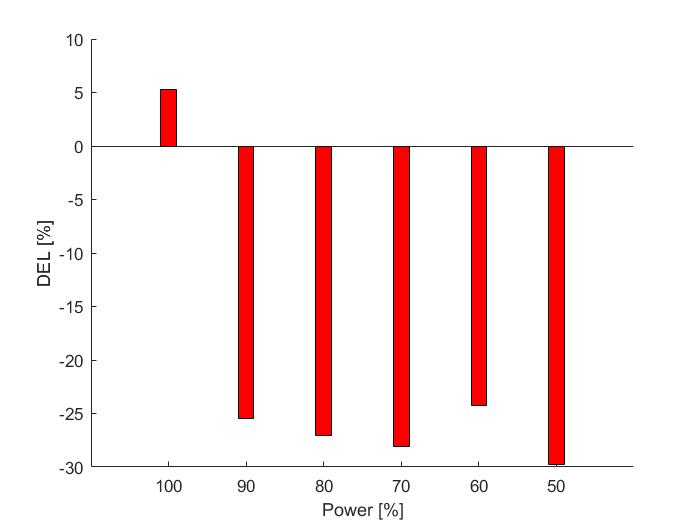
\includegraphics[width=\linewidth]{./Figures/trendPlot.jpg}
	\caption{DEL values for different $P_{ref}$}
	\label{fig:optimizationTrends}
\end{figure}
         
\section{Conclusion, Discussion and Recommendations}
What have we done and how to interpret the results
\subsection{Conclusion}
Conclusion about the results, Power reduction by axial  induction and yaw control will lead to a reduction in the loads on the wind farm. 
 

\subsection{Discussion+Recommendations}
This article which presents the results of an multi-objective wind farm optimization through yaw control and axial induction is bound to a number of limitations:
\begin{itemize}
	\item FLORIS, a low fidelity steady state model is used to calculate the flow in the wind farm. Turbulence and dynamic propagation of the wake as a consequence of turbine settings and the effect of wakes influencing each other are not implemented. Moreover, the the turbine determines its loads only for the most overlapping wake on the turbine, for the other wakes is a mean value taken. The effects in the wakes and the effect of multiple wakes on one turbine can have a significant influence on the loads and power of the turbine. Besides, should be mentioned that the effect of axial induction of the turbine is not applied to the loads but only to the power production of the turbine. 
	Our results for reference power tracking and load minimizations are only obtained from a three by three setup of wind turbines. Another setup or number of wind turbines may lead to other results. 
	\item FAST calculates the loads on the turbine based on a modeled inflow field which also does not take turbulence effects in the wake into account. The effect of dynamic propagation of the wake will lead to other load values. The shear effect on the wind speed of the inflow field is calculated for a reference height and  speed. Also the shear constant was set for a flat ocean ground surface. 
	The continuous wake profile uses only the velocity in the inner wake zone and the diameter of the outer wake zone from Gebraad. \cite{Gebraad2016} The partition of the wake in several wake zones with its own diameter and velocity is not longer implemented. For a sufficient model of the wake, a continuous function with more adjustable variables compared to one Gaussian should be considered.  
	\item The look-up-table with the DEL values is made for parameters with a certain step size. 
	\item   
\end{itemize}   



\begin{thebibliography}{99} % Bibliography - this is intentionally simple in this template

\bibitem{Nat2016}
Energieonderzoek Centrum Nederland. ''Nationale Energieverkenning 2016''

\bibitem{Tande2003}
J. O. G. Tande. "Grid integration of wind farms," in Wind Energy, 2003

\bibitem{Zalkind2016}
D. S. Zalkind and L. Y. Pao. "The fatigue loading effects of yaw control for wind plants," in American Control Conference (ACC), 2016
 
\bibitem{Fleming2014}
P. A. Fleming, P. M. Gebraad, S. Lee, J. W. van Wingerden, K. Johnson, M. Churchfield, P. Moriarty. ''Evaluating techniques for redirecting turbine wakes using SOWFA.'' in Renewable Energy, 2014

\bibitem{Hansen2014}
A. D. Hansen, P. Sørensen, F. Iov, F. Blaabjerg. ''Centralised power control of wind farm with doubly fed induction generators.'' in Renewable Energy, 2005

\bibitem{Boersma2017} 
S. Boersma, B. M. Doekemeijer, P. M. O. Gebraad, P. A. Fleming, J. Annoni,
A. K. Scholbrock, J. A. Frederik, and J-W. van Wingerden. ''A Tutorial on Control-Oriented Modeling and Control of Wind Farms,''
prsented at the American Control Conference, 2017


\bibitem{Kanev2017} 
S. K. Kanev and F. J. Savenije. "Active wake control: loads trends," in Wind Energy, 2017

\bibitem{Wilson2017}
B. Wilson. "Wind Farm Control: Robust Multi-Objective Optimization of a Wind Farm for Different Control Strategies," Unpublished Master's Thesis, 2017

\bibitem{Dijk2016}
M. T. van Dijk, J. W. van Wingerden, T. Ashuri, Y. Li, and M. A. Rotea. "Yaw-Misalignment and its Impact on Wind Turbine Loads and Wind Farm Power Output," in Journal of Physics: Conference Series, 2016

\bibitem{Bastankhah2016}
M. Bastankhah and F. Porte-Agel. "Experimental and theoretical study of wind turbine wakes in yawed conditions," in Journal of Fluid Mechanics, 2016

\bibitem{Gebraad2016}
P. M. O. Gebraad, F. W. Teeuwisse, J. W. Wingerden, P. A. Fleming, S. D. Ruben, J. R. Marden and L. Y. Pao. "Wind plant power optimization through yaw control using a parametric model for wake effects-a CFD simulation study," in Wind Energy, 2016

\bibitem{Jonkman2005}
J. M. Jonkman and M. L. Buhl Jr. "FAST User's Guide,'' National Renewable Energy Laboratory, Golden, CO, Technical Report No. NREL/EL-500-38230, 2005

\bibitem{Firtin2011}
E. Firtin, O. Guler, and S. A. Akdag. "Investigation of wind shear coefficients and their effect on electrical energy generation," in Applied Energy, 2011

\bibitem{Chougule2016}
A. Chougule, S. T. Kandukuri, and H.-G. Beyer. "Assessment of synthetic winds through spectral modeling and validation using FAST." Journal of Physics: Conference Series. Vol. 753. No. 4. IOP Publishing, 2016

\bibitem{Marden2013}
J. R. Marden, D. R. Shalom, and L. Y. Pao. "A model-free approach to wind farm control using game theoretic methods." IEEE Transactions on Control Systems Technology 21.4 (2013): 1207-1214	


\bibitem{vanDijk2016}
M. van Dijk. ''A Study on Yaw-Misaligment: Combined Optimization of Wind Farm Power Production and Structural Loading,'' Unpublished Master's Thesis, 2016

\bibitem{EWEA2016}
EWEA. ''Wind in power, 2015 European statistics,'' 2016

\bibitem{Jonkman2009}
J. M. Jonkman, S. Butterfield, W. Musial, and G. Scott. "Definition of a 5-MW Reference	Wind Turbine for Offshore System Development," National Renewable Energy Laboratory, 2009

\bibitem{Mlife}
 Mlife!!!!!!!!! nog juist refereren







\end{thebibliography}	
				
\end{document}
